


\begin{figure}[t]%h!
    \centering
    \begin{subfigure}{.47\textwidth}
        \centering
        %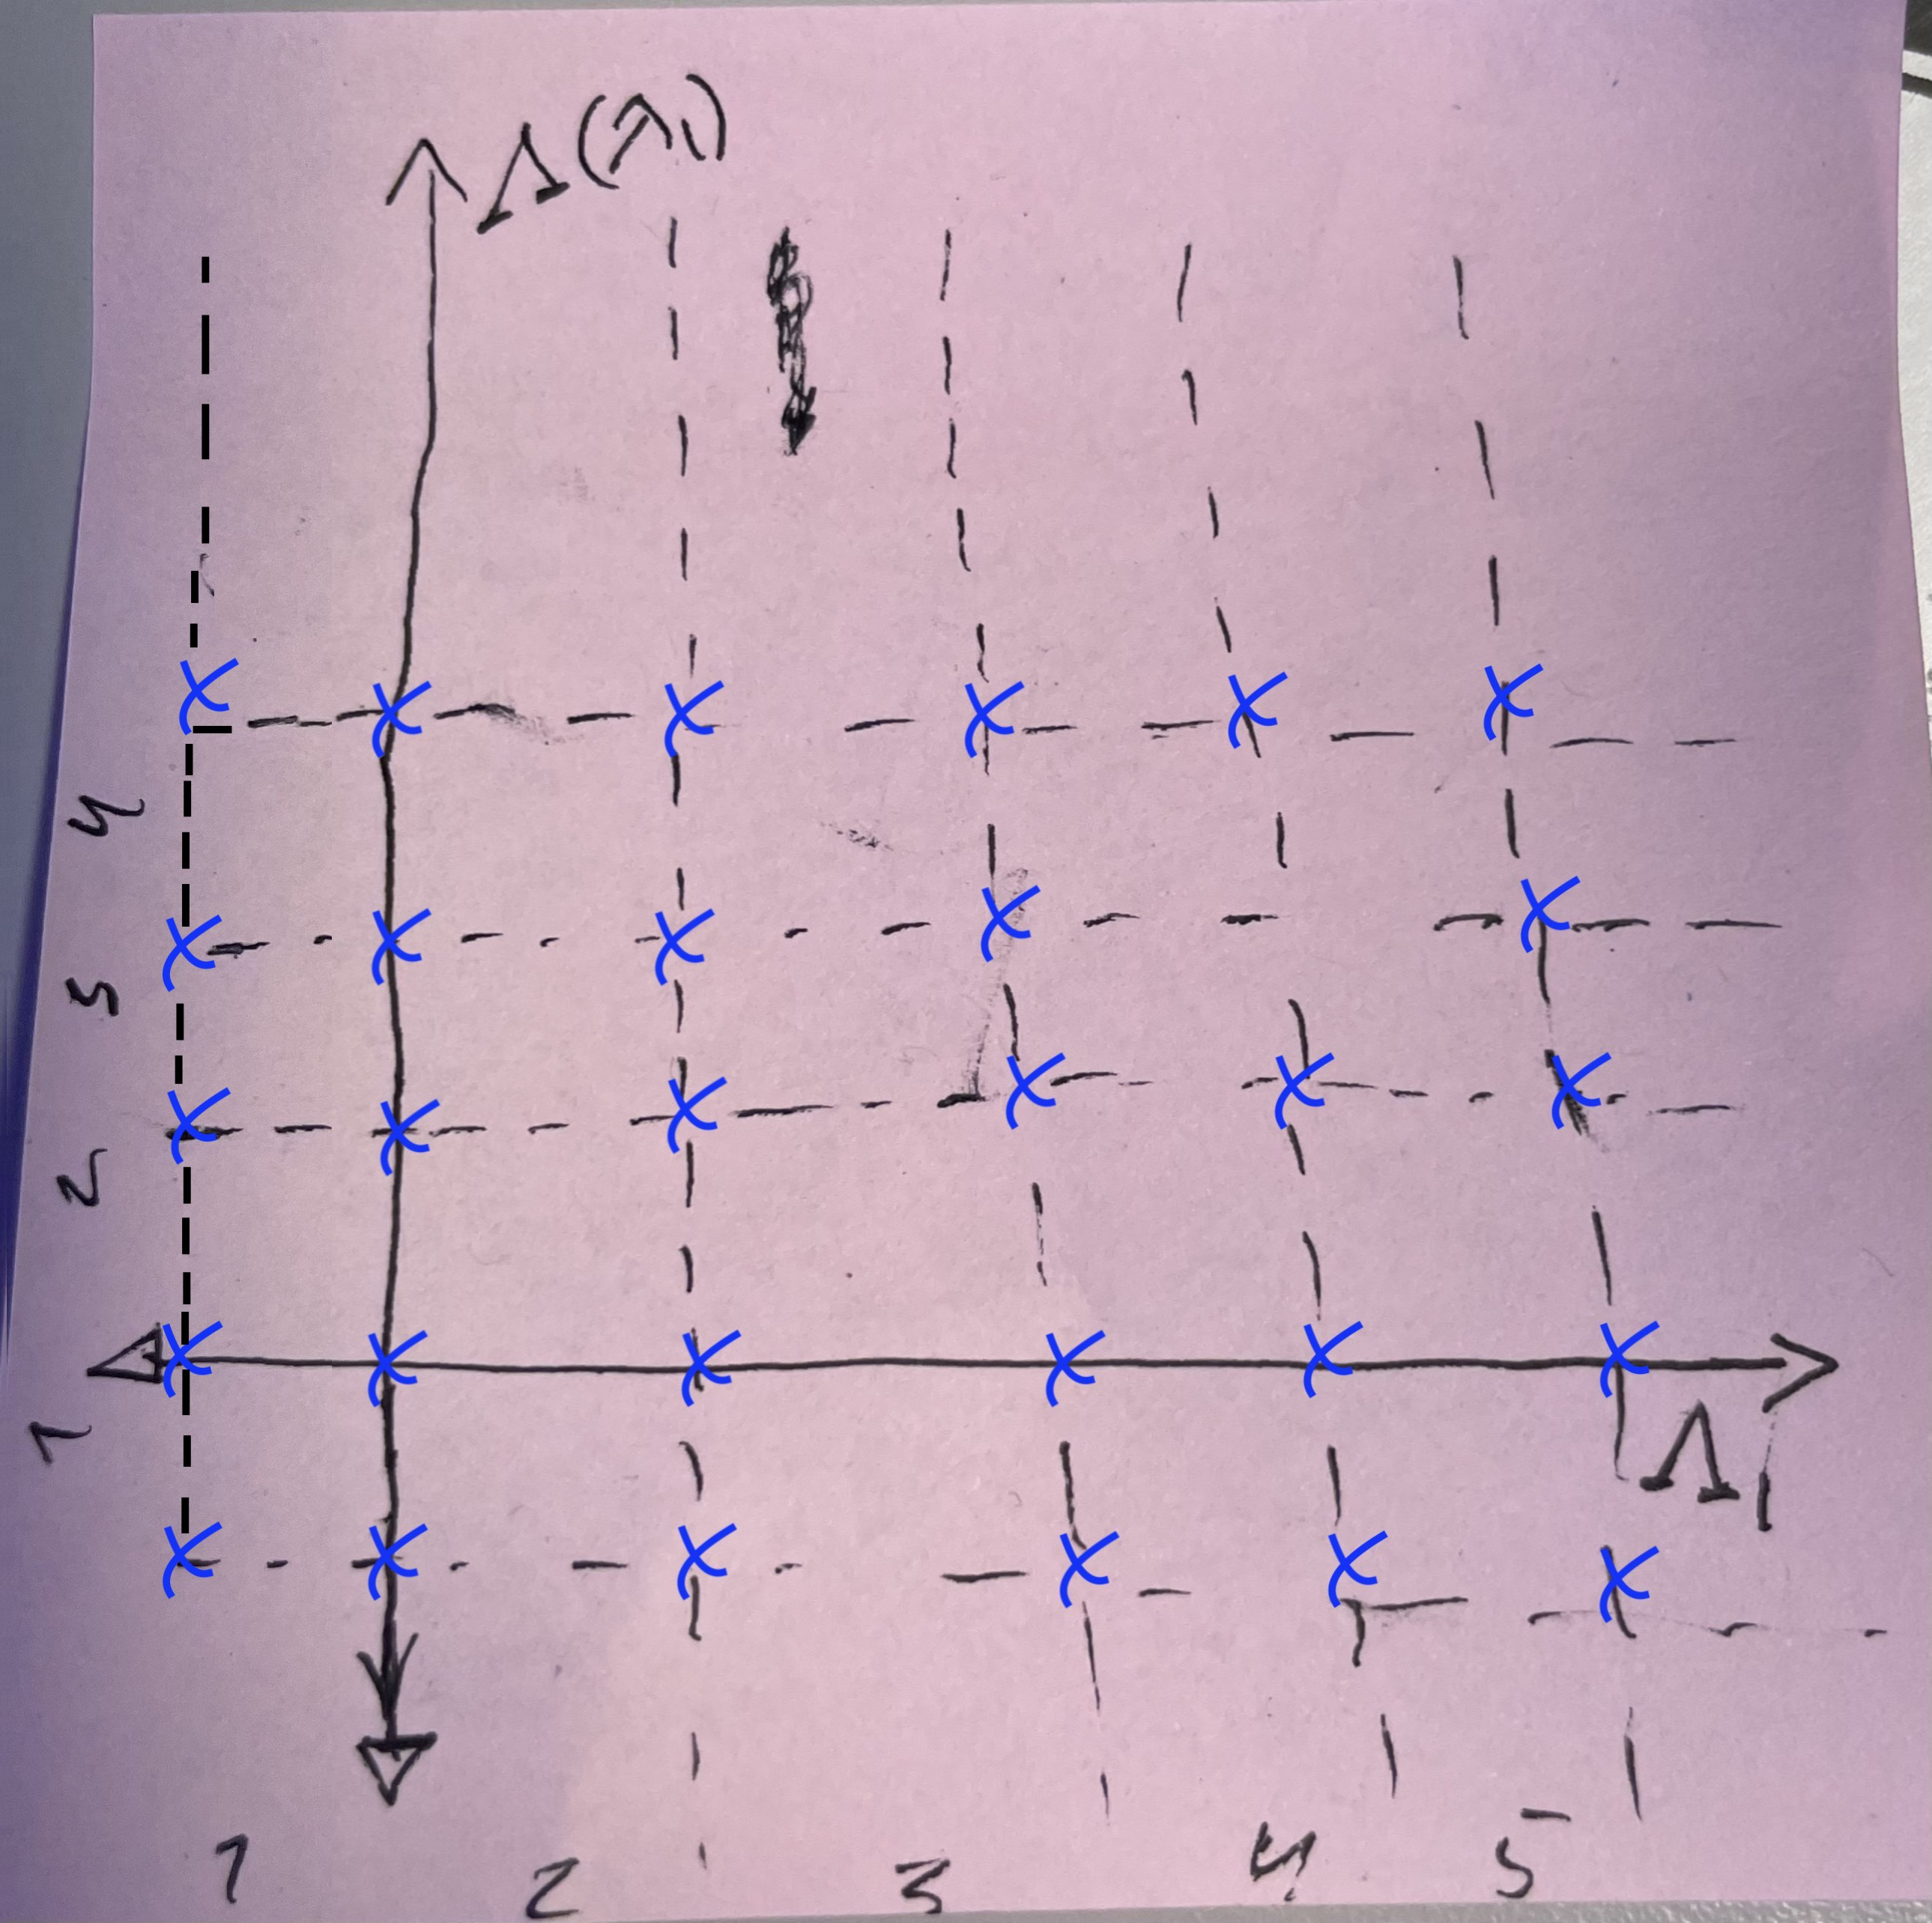
\includegraphics[width=0.9\linewidth]{spec_no_shift.jpg}
        %* Figure 1
        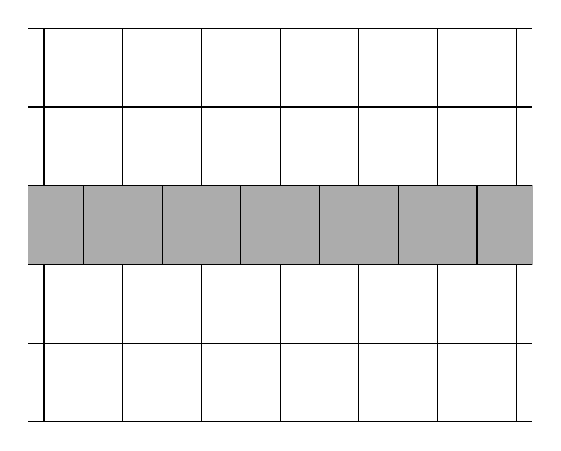
\begin{tikzpicture}[scale=1]
            % Define the tile
            \def\tile{
            \draw[fill=white] (0,0) rectangle (1,1);
            }
            \def\tiletwo{
            \draw[fill=gray!65] (0,0) rectangle (1,1);
            }
            
            % Draw the tiling pattern
            % Everything else
            \foreach \y in {0,1,3,4}{
                \foreach \x in {0,1,2,3,4,5}{
                    \pgfmathsetmacro{\shiftX}{\x} % Set horizontal shift
                    \pgfmathsetmacro{\shiftY}{\y}
                    \begin{scope}[shift={(\shiftX,\shiftY)}]
                        \tile
                    \end{scope}
                }
            }
            % Shifted line
            \foreach \x in {0}{
            \draw[gray!65, fill=gray!65] (\x-0.2,2) rectangle (\x+0.5,3);
            }
            \foreach \x in {6}{
            \draw[gray!65, fill=gray!65] (\x+0.2,2) rectangle (\x-0.5,3);
            }
            % Middle line, must be after the above code in order to get black lines at correct spots
            \foreach \y in {2}{
                \foreach \x in {0,1,2,3,4}{
                    \pgfmathsetmacro{\shiftX}{\x+0.5} % Set horizontal shift
                    \pgfmathsetmacro{\shiftY}{\y}
                    \begin{scope}[shift={(\shiftX,\shiftY)}]
                        \tiletwo
                    \end{scope}
                }
            }
            % small black lines at the top and bottom
            \foreach \y in {0,1,2,3,4,5}{
                \draw (0-0.2,\y) -- (6+0.2,\y);
            }
        \end{tikzpicture}
        %* —————————————————
        \caption{Single row shift}
        \label{fig:single_shift_horizontal_tiling}
    \end{subfigure}\quad
    \begin{subfigure}{.47\textwidth}
        \centering
        %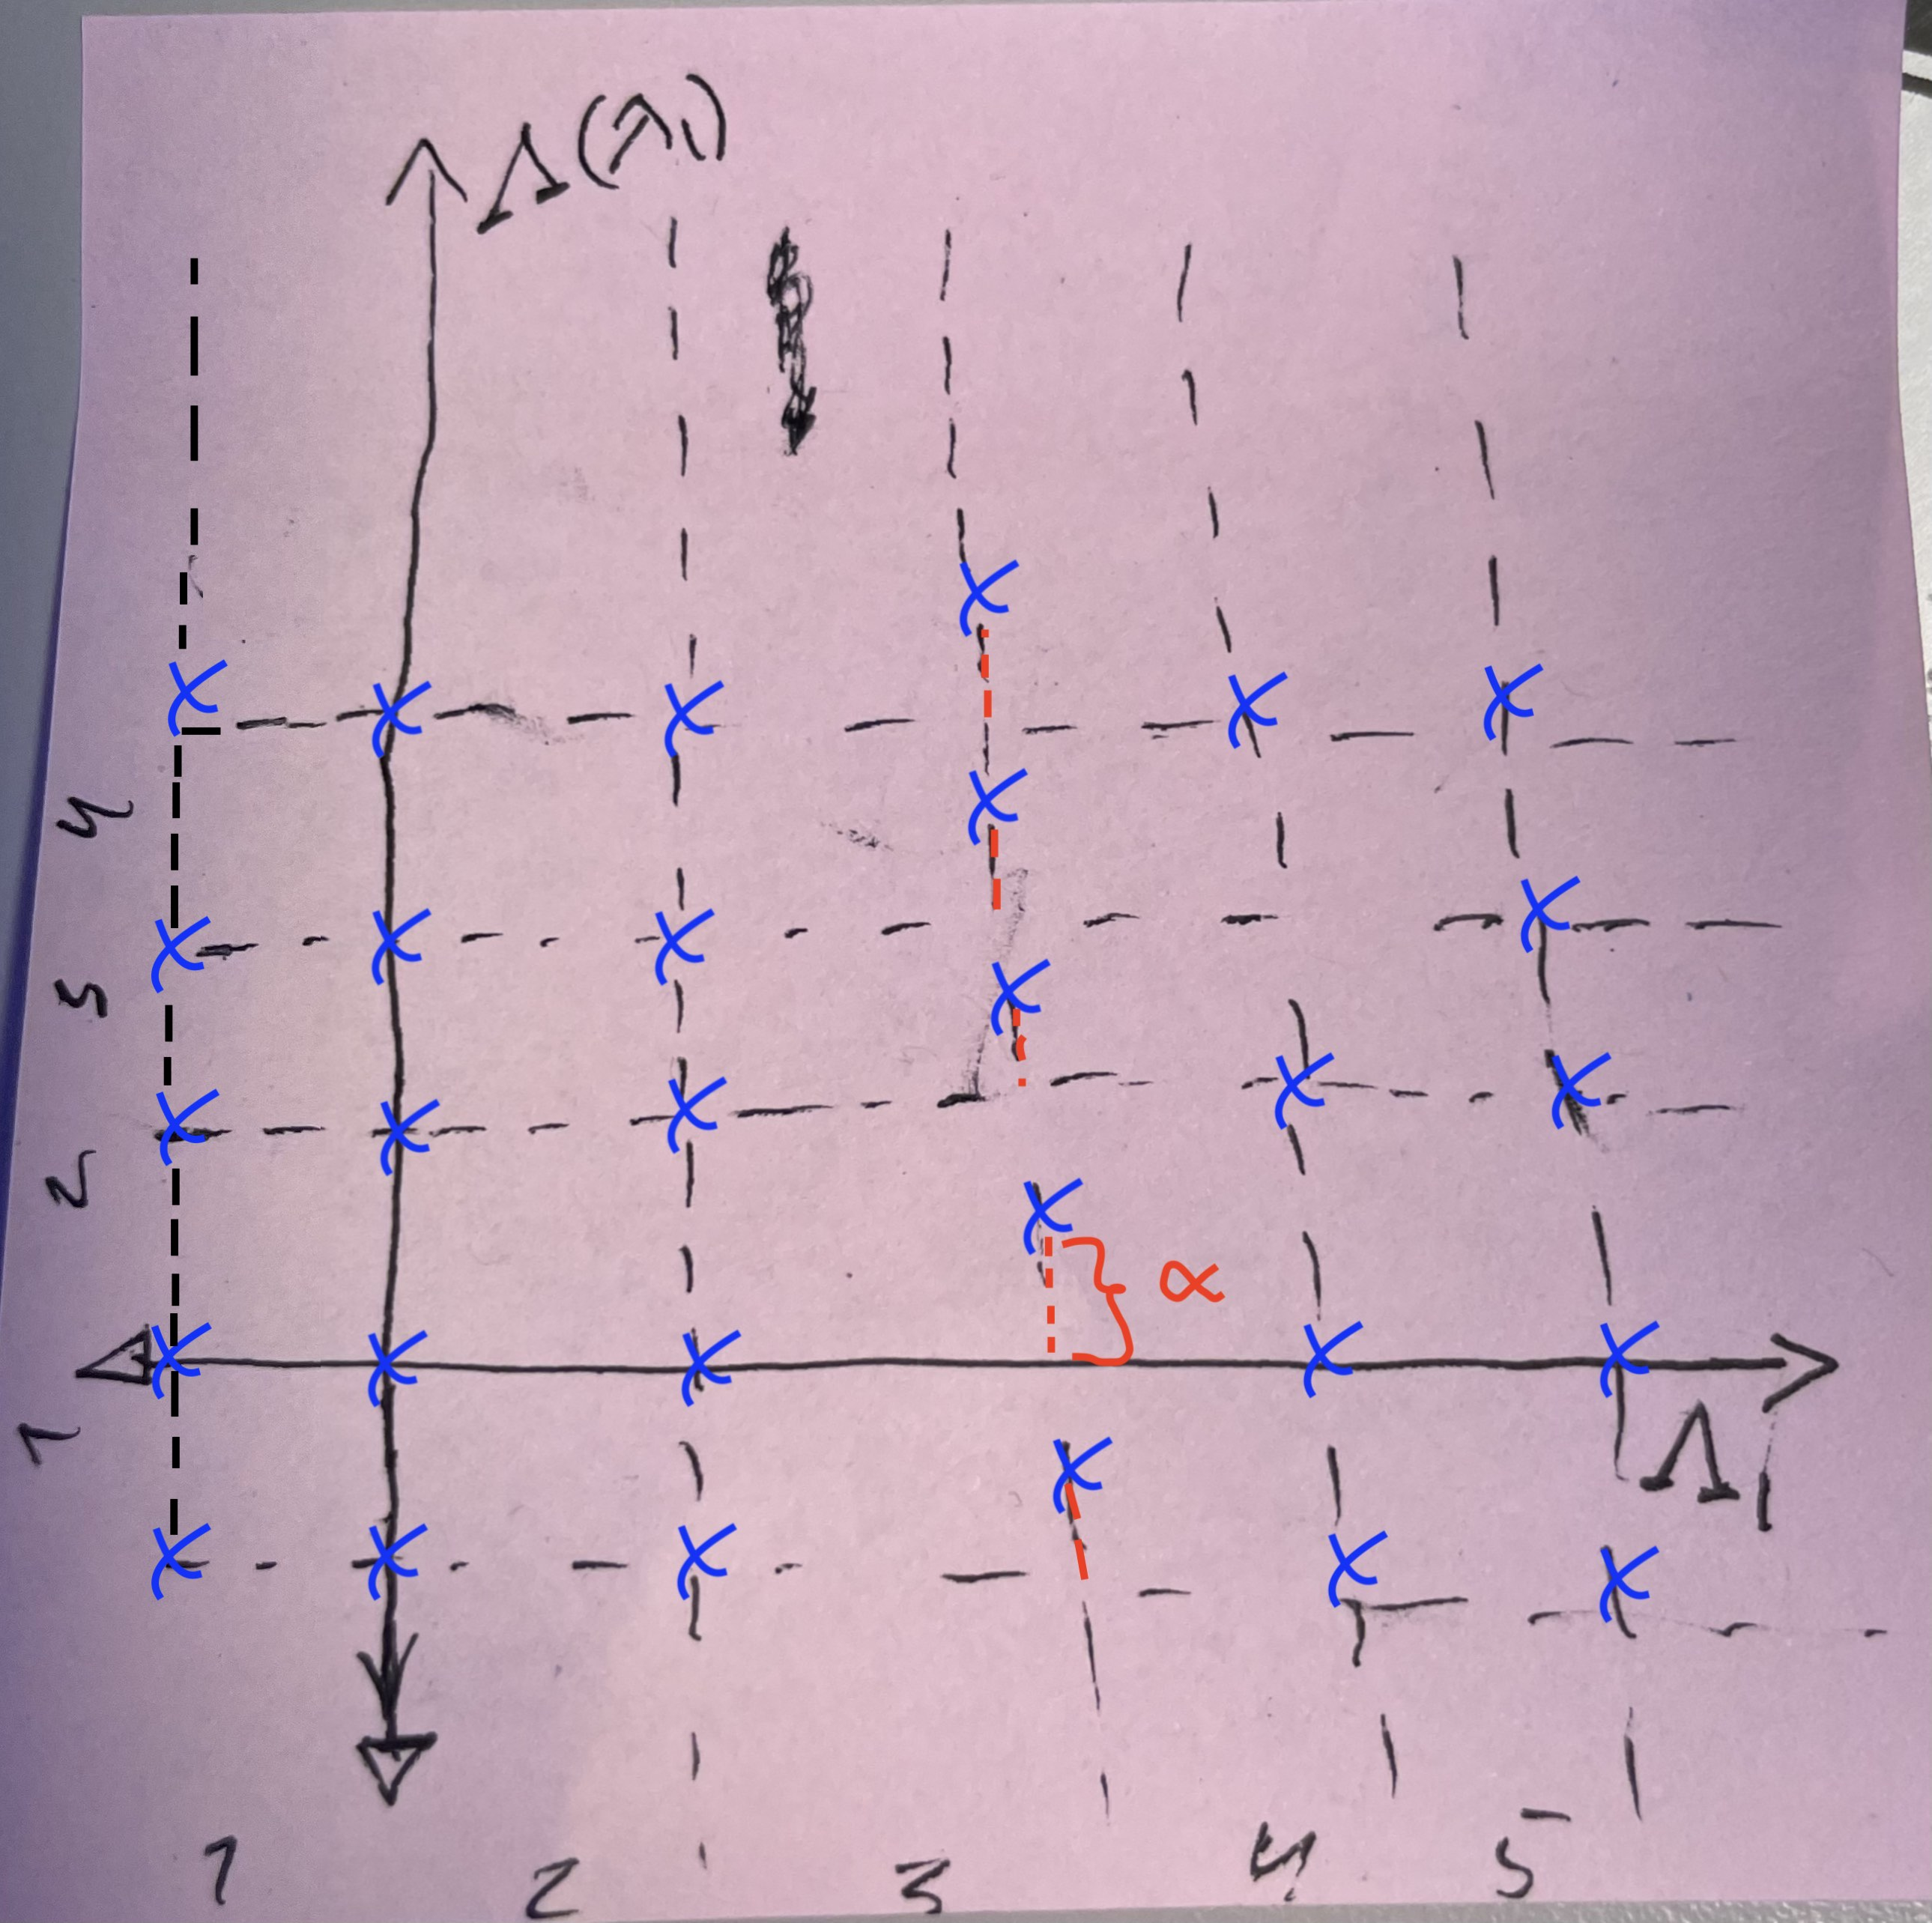
\includegraphics[width=0.9\linewidth]{spec_single_shift.jpg}
        %* Figure 2
        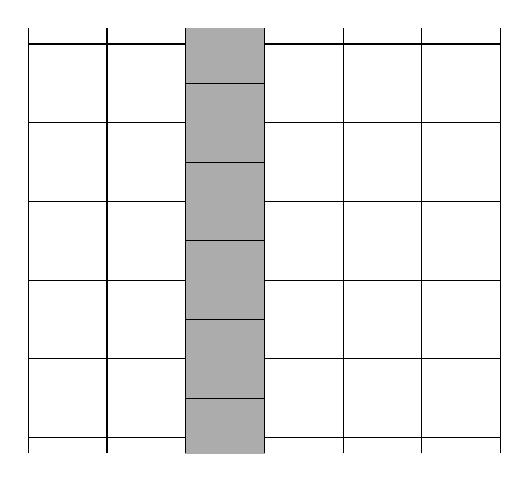
\begin{tikzpicture}[scale=1]
            % Define the tile
            \def\tile{
            \draw[fill=white] (0,0) rectangle (1,1);
            }
            \def\tiletwo{
            \draw[fill=gray!65] (0,0) rectangle (1,1);
            }
            
            % Draw the tiling pattern
            % Everything else
            \foreach \x in {0,1,3,4,5}{
                \foreach \y in {0,1,2,3,4}{
                    \pgfmathsetmacro{\shiftX}{\x} % Set horizontal shift
                    \pgfmathsetmacro{\shiftY}{\y}
                    \begin{scope}[shift={(\shiftX,\shiftY)}]
                        \tile
                    \end{scope}
                }
            }
            % Shifted line
            \foreach \y in {0}{
            \draw[gray!65, fill=gray!65] (2,\y-0.2) rectangle (3,\y+0.5);
            }
            \foreach \y in {5}{
            \draw[gray!65, fill=gray!65] (2,\y+0.2) rectangle (3,\y-0.5);
            }
            % Middle line, must be after the above code in order to get black lines at correct spots
            \foreach \x in {2}{
                \foreach \y in {0,1,2,3}{
                    \pgfmathsetmacro{\shiftX}{\x} % Set horizontal shift
                    \pgfmathsetmacro{\shiftY}{\y+0.5}
                    \begin{scope}[shift={(\shiftX,\shiftY)}]
                        \tiletwo
                    \end{scope}
                }
            }
            % small black lines at the top and bottom
            \foreach \x in {0,1,2,3,4,5,6}{
                \draw (\x,0-0.2) -- (\x,5+0.2);
            }
        \end{tikzpicture}
        %* —————————————————
        \caption{Single column shift}
        \label{fig:single_shift_vertical_tiling}
    \end{subfigure}\\
    \begin{subfigure}{.47\textwidth}
        \centering
        %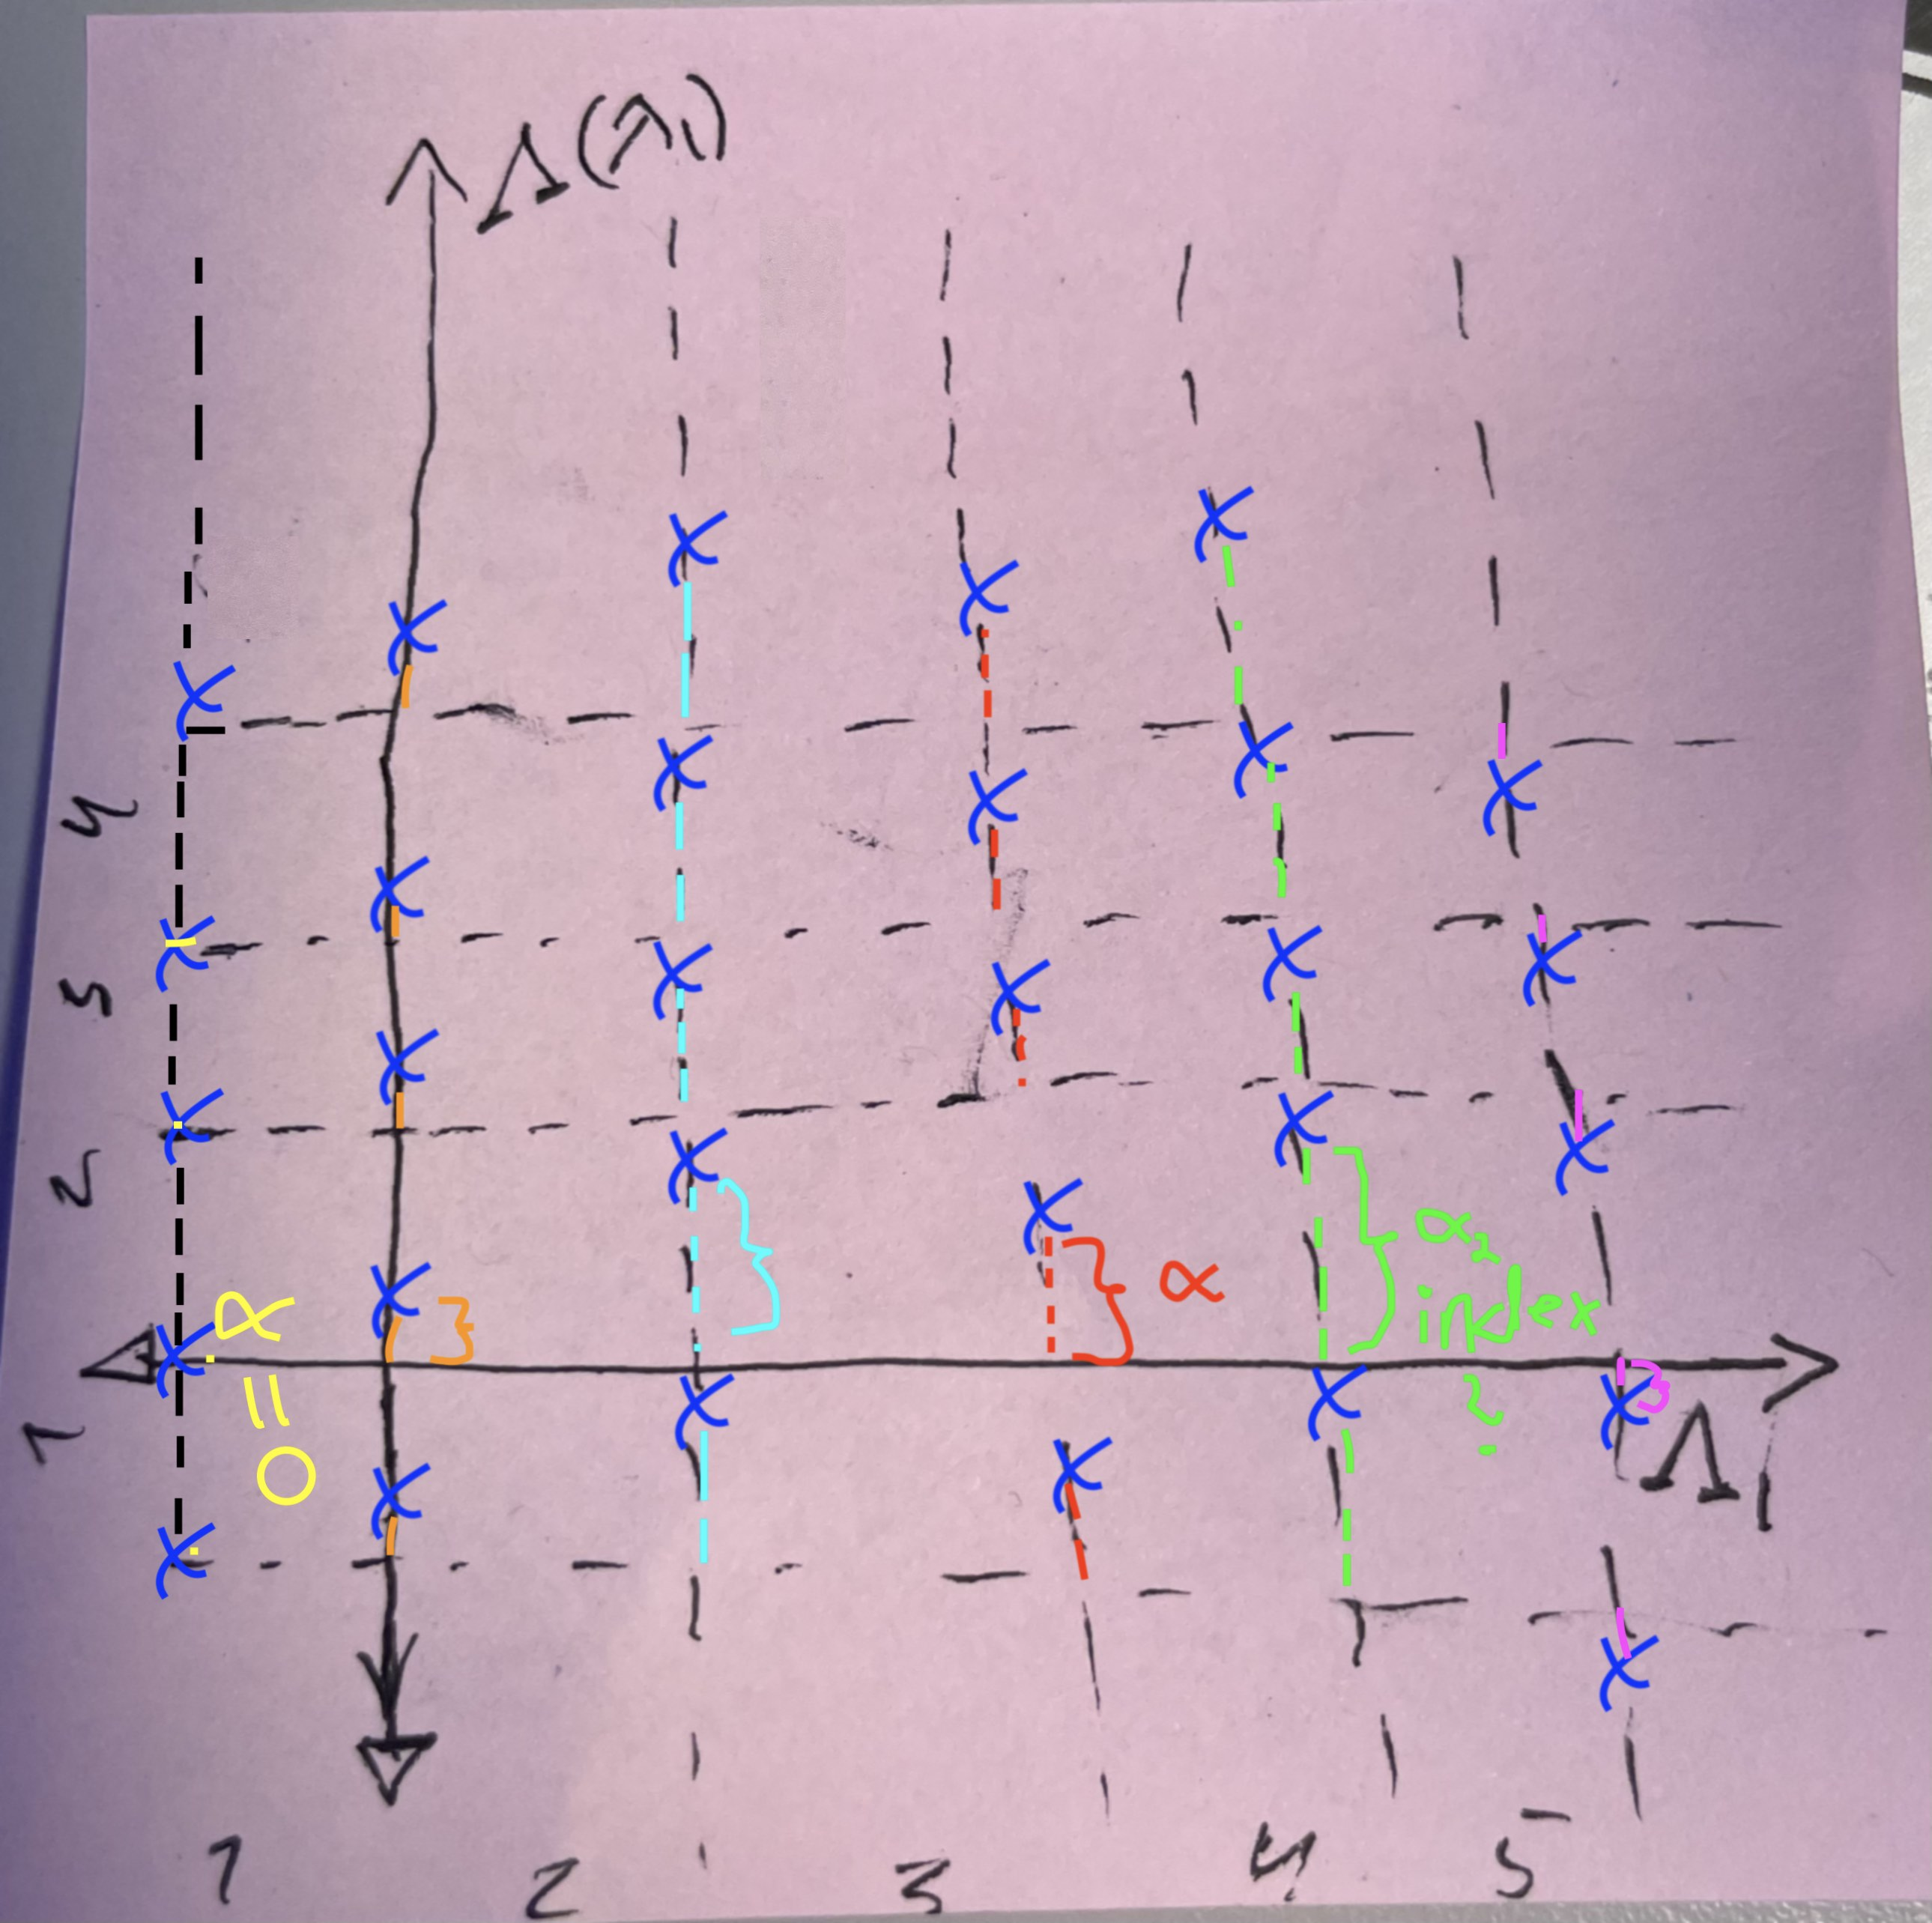
\includegraphics[width=0.9\linewidth]{multiple_shift_left_zero.jpg}
        %* Figure 3
        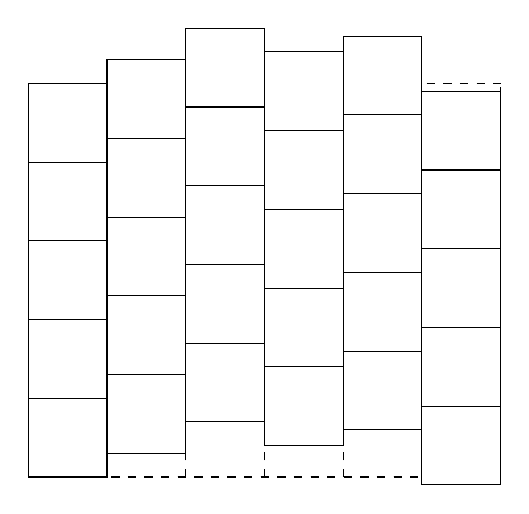
\begin{tikzpicture}[scale=1]
            % Define the tile
            \def\tile{
            % Draw the unit square
            \draw[fill=white] (0,0) rectangle (1,1);
            }

            % Shift list
            \def\BetaMinOne{0}
            \def\BetaZero{0.3}
            \def\BetaOne{0.7}
            \def\BetaTwo{0.4}
            \def\BetaThree{0.6}
            \def\BetaFour{-0.1}
            
            

% Axis lines
%\draw[->] (-1.5,0) -- (4.5,0) node[right] {$X$};
%\draw[->] (0,-1.5) -- (0,3.5) node[above] {$Y$};
\draw[dashed] (0,0) -- (6,0);
\draw[dashed] (0,0) -- (0,5);

% Dashed lines at each integer in the x direction
\foreach \x in {0,...,6}
    \draw[dashed] (\x,0) -- (\x,5);

% Dashed lines at each integer in the y direction
\foreach \y in {0,...,5}
    \draw[dashed] (0,\y) -- (6,\y);


            % Draw the tiling pattern
            \foreach \x in {0,1,2,3,4,5}{
            \foreach \y in {0,1,2,3,4}{
                \ifnum\x=0 % Set vertical shift for the third column only
                    \pgfmathsetmacro{\shiftX}{\x} % No vertical shift for other columns
                    \pgfmathsetmacro{\shiftY}{\y + \BetaMinOne} % Shift one unit upward
                \fi
                \ifnum\x=1
                    \pgfmathsetmacro{\shiftX}{\x}
                    \pgfmathsetmacro{\shiftY}{\y + \BetaZero}
                \fi
                \ifnum\x=2
                    \pgfmathsetmacro{\shiftX}{\x} 
                    \pgfmathsetmacro{\shiftY}{\y + \BetaOne} 
                \fi
                \ifnum\x=3
                    \pgfmathsetmacro{\shiftX}{\x}
                    \pgfmathsetmacro{\shiftY}{\y + \BetaTwo}
                \fi
                \ifnum\x=4
                    \pgfmathsetmacro{\shiftX}{\x}
                    \pgfmathsetmacro{\shiftY}{\y + \BetaThree}
                \fi
                \ifnum\x=5
                    \pgfmathsetmacro{\shiftX}{\x}
                    \pgfmathsetmacro{\shiftY}{\y + \BetaFour}
                \fi
                \begin{scope}[shift={(\shiftX,\shiftY)}]
                \tile % Draw the tile
                \end{scope}
            }}
        \end{tikzpicture}
        %* —————————————————
        \caption{Multiple shifts vertical}
        \label{fig:multiple_shift_vertical_tiling}
    \end{subfigure}\quad
    \begin{subfigure}{.47\textwidth}
        \centering
        %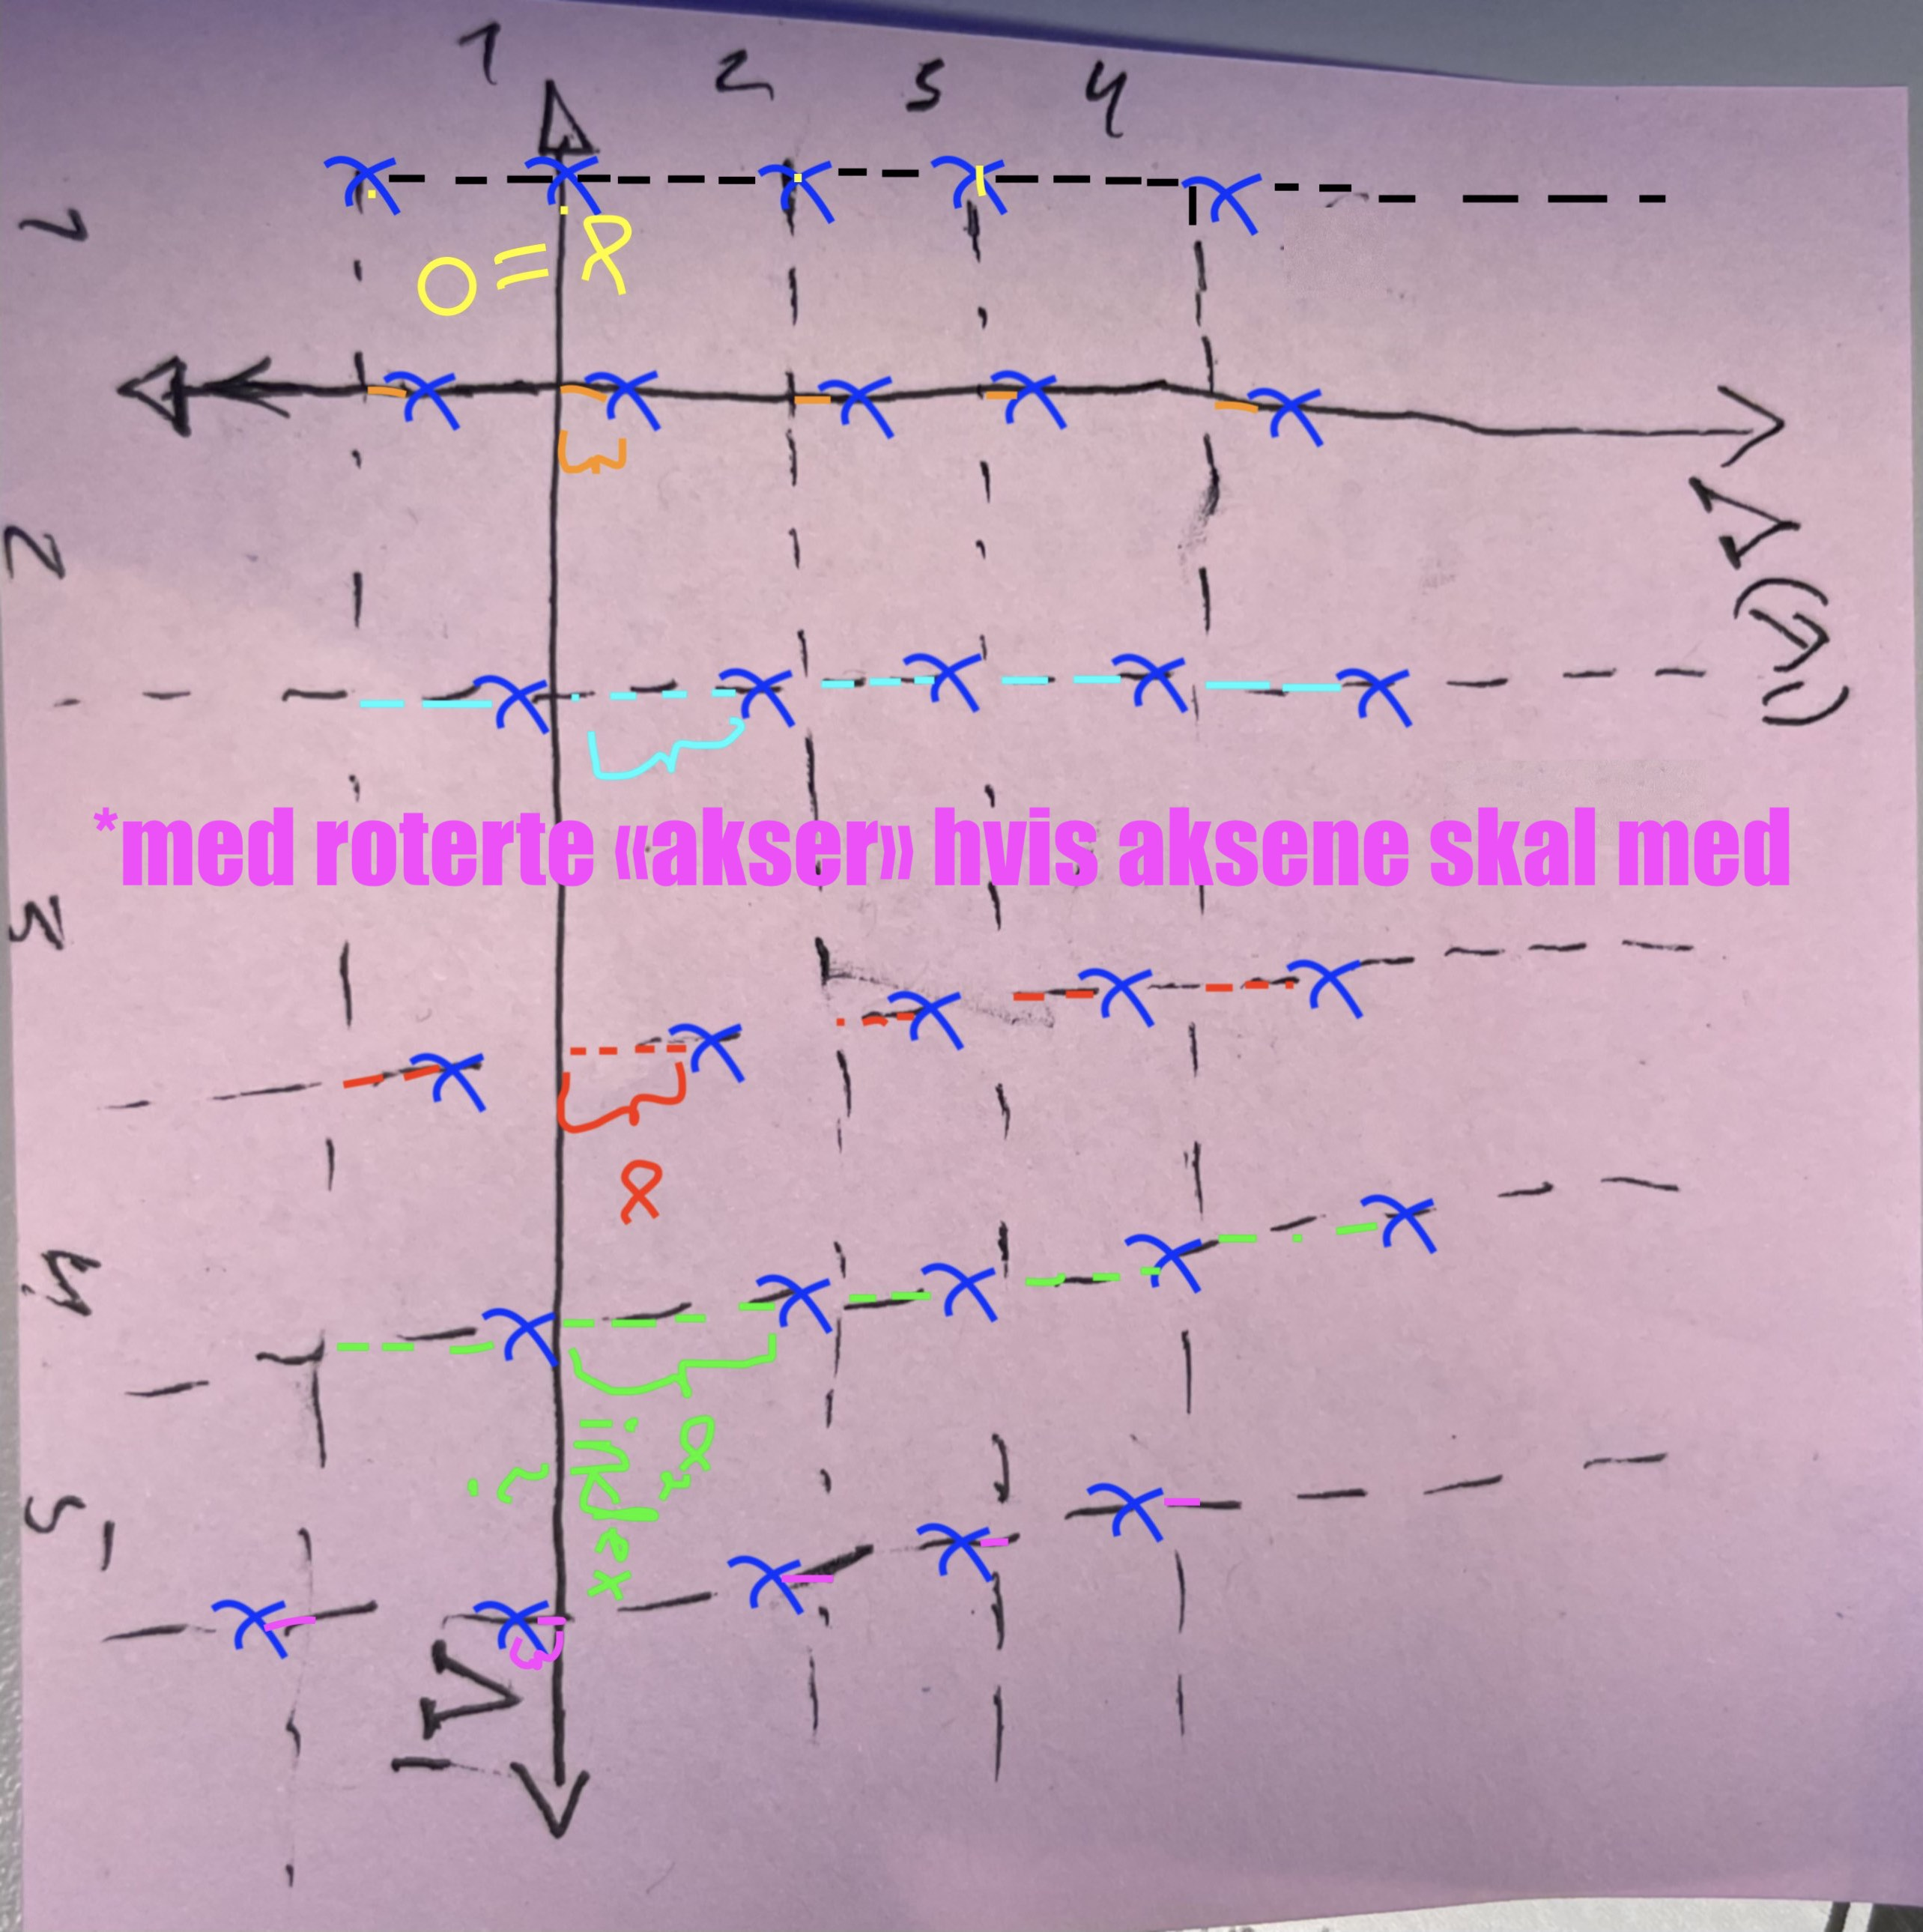
\includegraphics[width=0.9\linewidth]{multiple_shift_left_zero_horizontal.jpg}
        %* Figure 4
        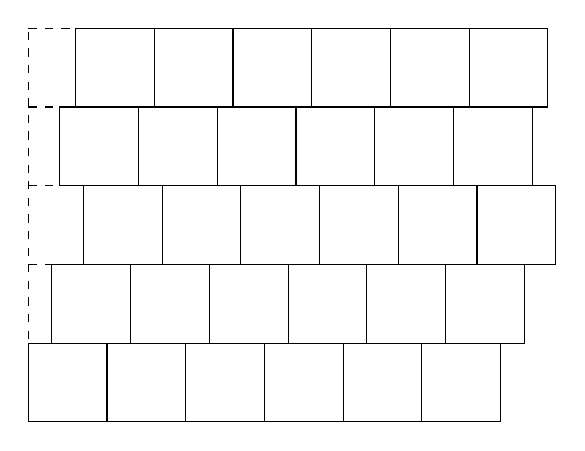
\begin{tikzpicture}[scale=1]
            % Define the tile
            \def\tile{
            % Draw the unit square
            \draw[fill=white] (0,0) rectangle (1,1);
            }

            % Shift list
            \def\BetaMinOne{0}
            \def\BetaZero{0.3}
            \def\BetaOne{0.7}
            \def\BetaTwo{0.4}
            \def\BetaThree{0.6}
            
            

% Axis lines
%\draw[->] (-1.5,0) -- (4.5,0) node[right] {$X$};
%\draw[->] (0,-1.5) -- (0,3.5) node[above] {$Y$};
\draw[dashed] (0,0) -- (6,0);
\draw[dashed] (0,0) -- (0,5);

% Dashed lines at each integer in the x direction
\foreach \x in {0,...,6}
    \draw[dashed] (\x,0) -- (\x,5);

% Dashed lines at each integer in the y direction
\foreach \y in {0,...,5}
    \draw[dashed] (0,\y) -- (6,\y);


            % Draw the tiling pattern
            \foreach \x in {0,1,2,3,4,5}{
            \foreach \y in {0,1,2,3,4}{
                \ifnum\y=0
                    \pgfmathsetmacro{\shiftX}{\x + \BetaMinOne}
                    \pgfmathsetmacro{\shiftY}{\y}
                \fi
                \ifnum\y=1
                    \pgfmathsetmacro{\shiftX}{\x + \BetaZero}
                    \pgfmathsetmacro{\shiftY}{\y}
                \fi
                \ifnum\y=2
                    \pgfmathsetmacro{\shiftX}{\x + \BetaOne} 
                    \pgfmathsetmacro{\shiftY}{\y} 
                \fi
                \ifnum\y=3
                    \pgfmathsetmacro{\shiftX}{\x + \BetaTwo}
                    \pgfmathsetmacro{\shiftY}{\y}
                \fi
                \ifnum\y=4
                    \pgfmathsetmacro{\shiftX}{\x + \BetaThree}
                    \pgfmathsetmacro{\shiftY}{\y}
                \fi
                \begin{scope}[shift={(\shiftX,\shiftY)}]
                \tile % Draw the tile
                \end{scope}
            }}
        \end{tikzpicture}
        %* —————————————————
        \caption{Multiple shifts horizontal}
        \label{fig:multiple_shift_horizontal_tiling}
    \end{subfigure}
    \caption{Text}
    \label{fig:tiling_figures}
\end{figure}
